\documentclass{beamer}
\usepackage{fontspec}
\usepackage{graphicx}
\usepackage{subcaption}
\usepackage{hyperref}
% \usepackage{minted}
% \usepackage{listings}
\usepackage{polski}

% build logs whispered to me that it's not needed, but I'll keep it just in case
\usepackage[utf8]{inputenc} 
\usetheme{Copenhagen}

\title{Nix i NixOS}
\author{Viktor Grünwaldt}
\date{\today}

\begin{document}

\begin{frame}
    \titlepage
\end{frame}

\begin{frame}
    
\includegraphics[width=0.75\linewidth]{./assets/NixOS_logo.png}
\end{frame}

\begin{frame}{Wprowadzenie do NixOS}
    \begin{itemize}
        \item Historia i filozofia
        \item Deklaratywna konfiguracja
        \item Atomowe aktualizacje
    \end{itemize}
\end{frame}

\begin{frame}{Historia i filozofia}
    \begin{figure}
        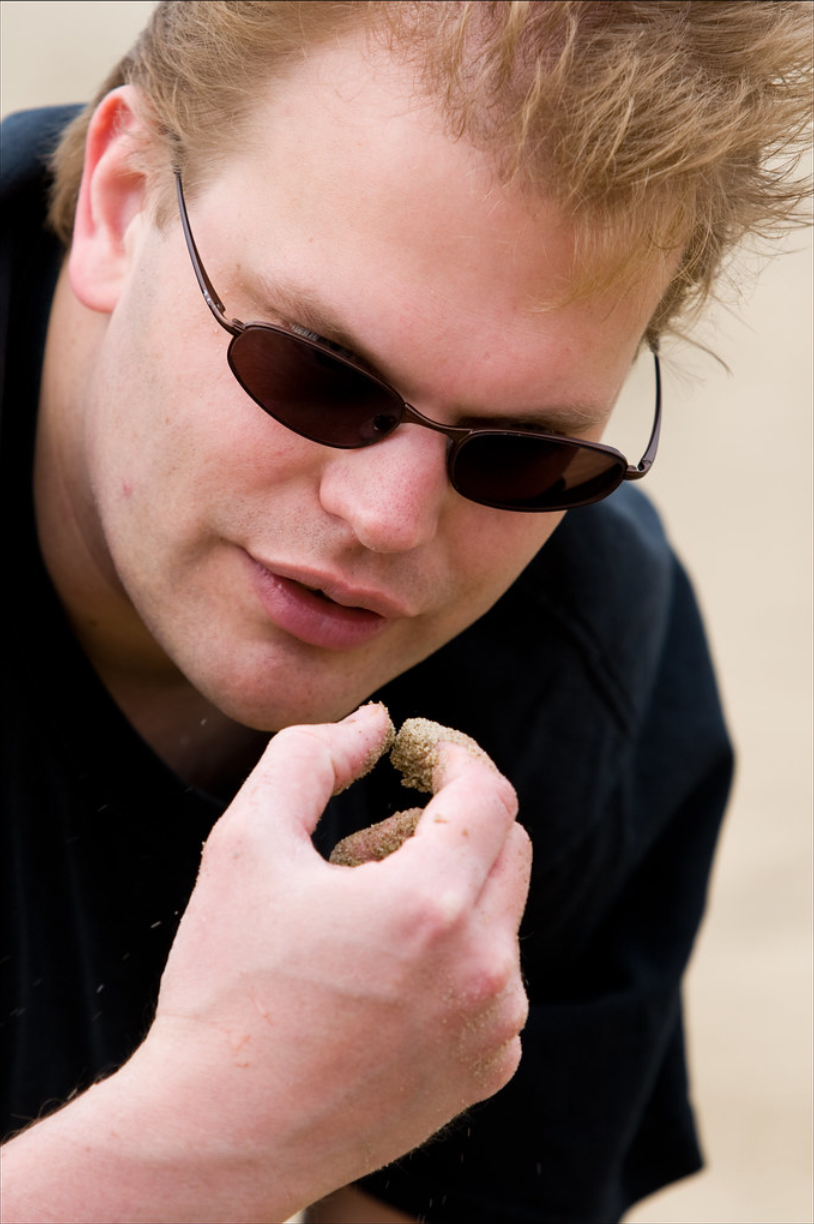
\includegraphics[height=0.75\textheight]{./assets/eelco.jpg}
        \caption*{\scriptsize Źródło: Eelco Visser, Flickr, \url{https://www.flickriver.com/photos/eelcovisser/3618182654/}}
    \end{figure}
\end{frame}

\begin{frame}{Deklaratywna konfiguracja}
    \begin{figure}
        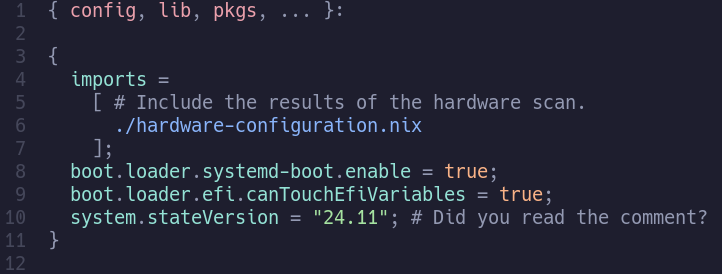
\includegraphics[width=\linewidth]{./assets/configuration.png}
        \caption*{\scriptsize Minimalna konfiguracja wygenerowana poleceniem \texttt{nixos-generate-config --dir .}}
    \end{figure}
\end{frame}

\begin{frame}{Nix - Menedżer pakietów}
    \begin{itemize}
        \item Functional package management
        \item Izolacja pakietów
        \item `/nix/store`
    \end{itemize}
\end{frame}

\begin{frame}{Deklaratywna konfiguracja systemu}
    \begin{itemize}
        \item Plik `configuration.nix`
        \item Usługi i pakiety
        \item Utrzymanie środowisk
    \end{itemize}
\end{frame}

\begin{frame}{System budowania i kompilowania}
    \begin{itemize}
        \item Derywacje
        \item Zależności i hermetyzacja
        \item Nie zmienność
    \end{itemize}
\end{frame}

\begin{frame}{Zaawansowane funkcje NixOS}
    \begin{itemize}
        \item Rollbacki systemowe
        \item Bezpieczne aktualizacje
        \item Wersje pakietów
    \end{itemize}
\end{frame}

\begin{frame}{Przykłady zastosowań NixOS}
    \begin{itemize}
        \item CI/CD
        \item Zarządzanie infrastrukturą
        \item Kontenery i VM
    \end{itemize}
\end{frame}

\begin{frame}{Zalety i wyzwania}
    \begin{itemize}
        \item Zalety: deterministyczne środowisko, stabilność
        \item Wyzwania: krzywa uczenia się, kompatybilność
    \end{itemize}
\end{frame}

\begin{frame}{Wyzwania: krzywa uczenia się}
    \begin{figure}
        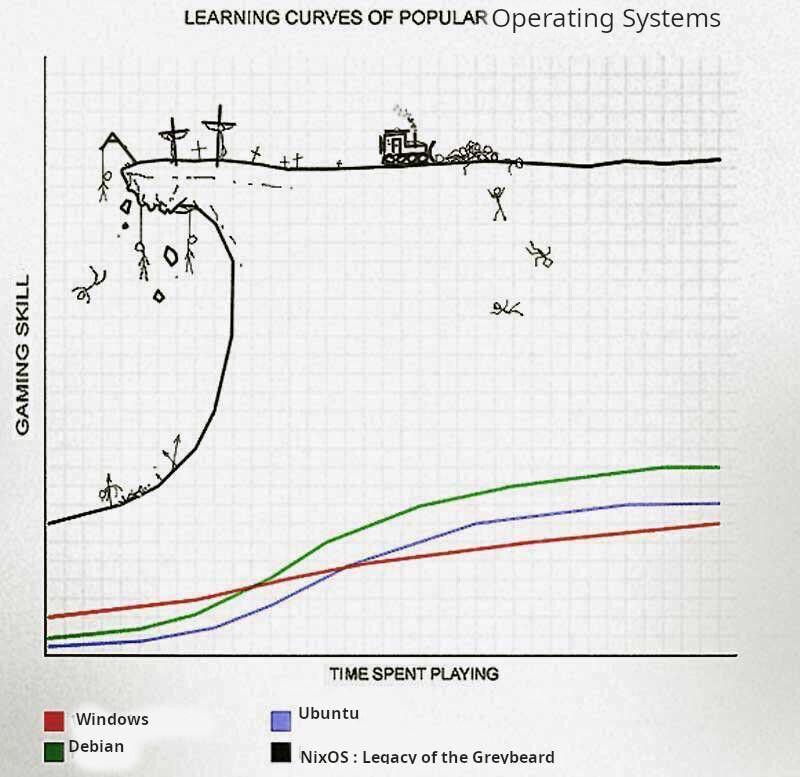
\includegraphics[width=0.75\linewidth, height=0.75\textheight]{./assets/nixoscurve.jpg}
        \caption*{\scriptsize Źródło: \url{https://discourse.nixos.org/t/probably-the-best-lecture-of-nix-fundamentals-on-the-internet/9893}} % Use caption* for non-numbered source text
    \end{figure}
\end{frame}

\begin{frame}{Narzędzia związane z NixOS}
    \begin{itemize}
        \item flake + experimental-cli
        \item disko
        \item nixos-anywhere
        \item home-manager
        \item lix/tvix
        \item guix
        \item nixos-alien
        \item nixos-sops
        \item nixos wiki
        \item nix pills
        \item zero to nix
        \item nix.dev
        \item nix manual
        \item official nixos wiki
        \item \{lang\}2nix
    \end{itemize}
\end{frame}

\begin{frame}{Narzędzia związane z NixOS 2}
    \begin{itemize}
        \item hydra
        \item nix shell
        \item nix develop
        \item nix build
        \item nix gc
        \item devenv
        \item devbox
        \item cachix
        \item overlays
        \item pins/npins
        \item nixpkgs
        \item nixbsd
        \item lanzaboote
    \end{itemize}
\end{frame}

\begin{frame}{Demo na żywo}
    \begin{itemize}
        \item Kompilacja `nano` za pomocą derywacji
        \item Niestandardowa derywacja
        \item `nixos-rebuild switch`
    \end{itemize}
\end{frame}

\begin{frame}{Podobne narzędzia}
    \begin{itemize}
        \item Ansible
        \item Docker
        \item Fedora Silverblue
        \item asdf, mise
        \item Flatpak, Appimage, Snap
        \item Brew
    \end{itemize}
\end{frame}

\begin{frame}{Podsumowanie i pytania}
    \begin{itemize}
        \item Podsumowanie korzyści NixOS
        \item Pytania
    \end{itemize}
\end{frame}

\end{document}
